\section{Der Anfang vom Anfang.}
    Der Text ist \underline{\textit{\textbf{"verhext"}}}, braucht kein Slash und keine Klammern, 
    das ist der Hammer(n).

    \enquote{Und dieser Text ist umgeben von Anführungszeichen.}
    
    
        Die Abbildung \ref{fig:DAVES_PANCAKES_RECIPE} zeigt das erleuterte Rezept
        in größerem Detail. 
        \newline
        Siehe Kapitel \ref{kapitel_02} \nameref{kapitel_02}

        % line break mit leerzeichen zwischen den zeilen! so easy!
        1.) zutaten

        2.) bearbeitungsweise

        3.) More Stuff

        \begin{figure}[H]
            \centering
            % error 'overfull' = bild zu groß für platz, fixed indem man width auf das 0.x Fache anpasst (hier 0.5) 
            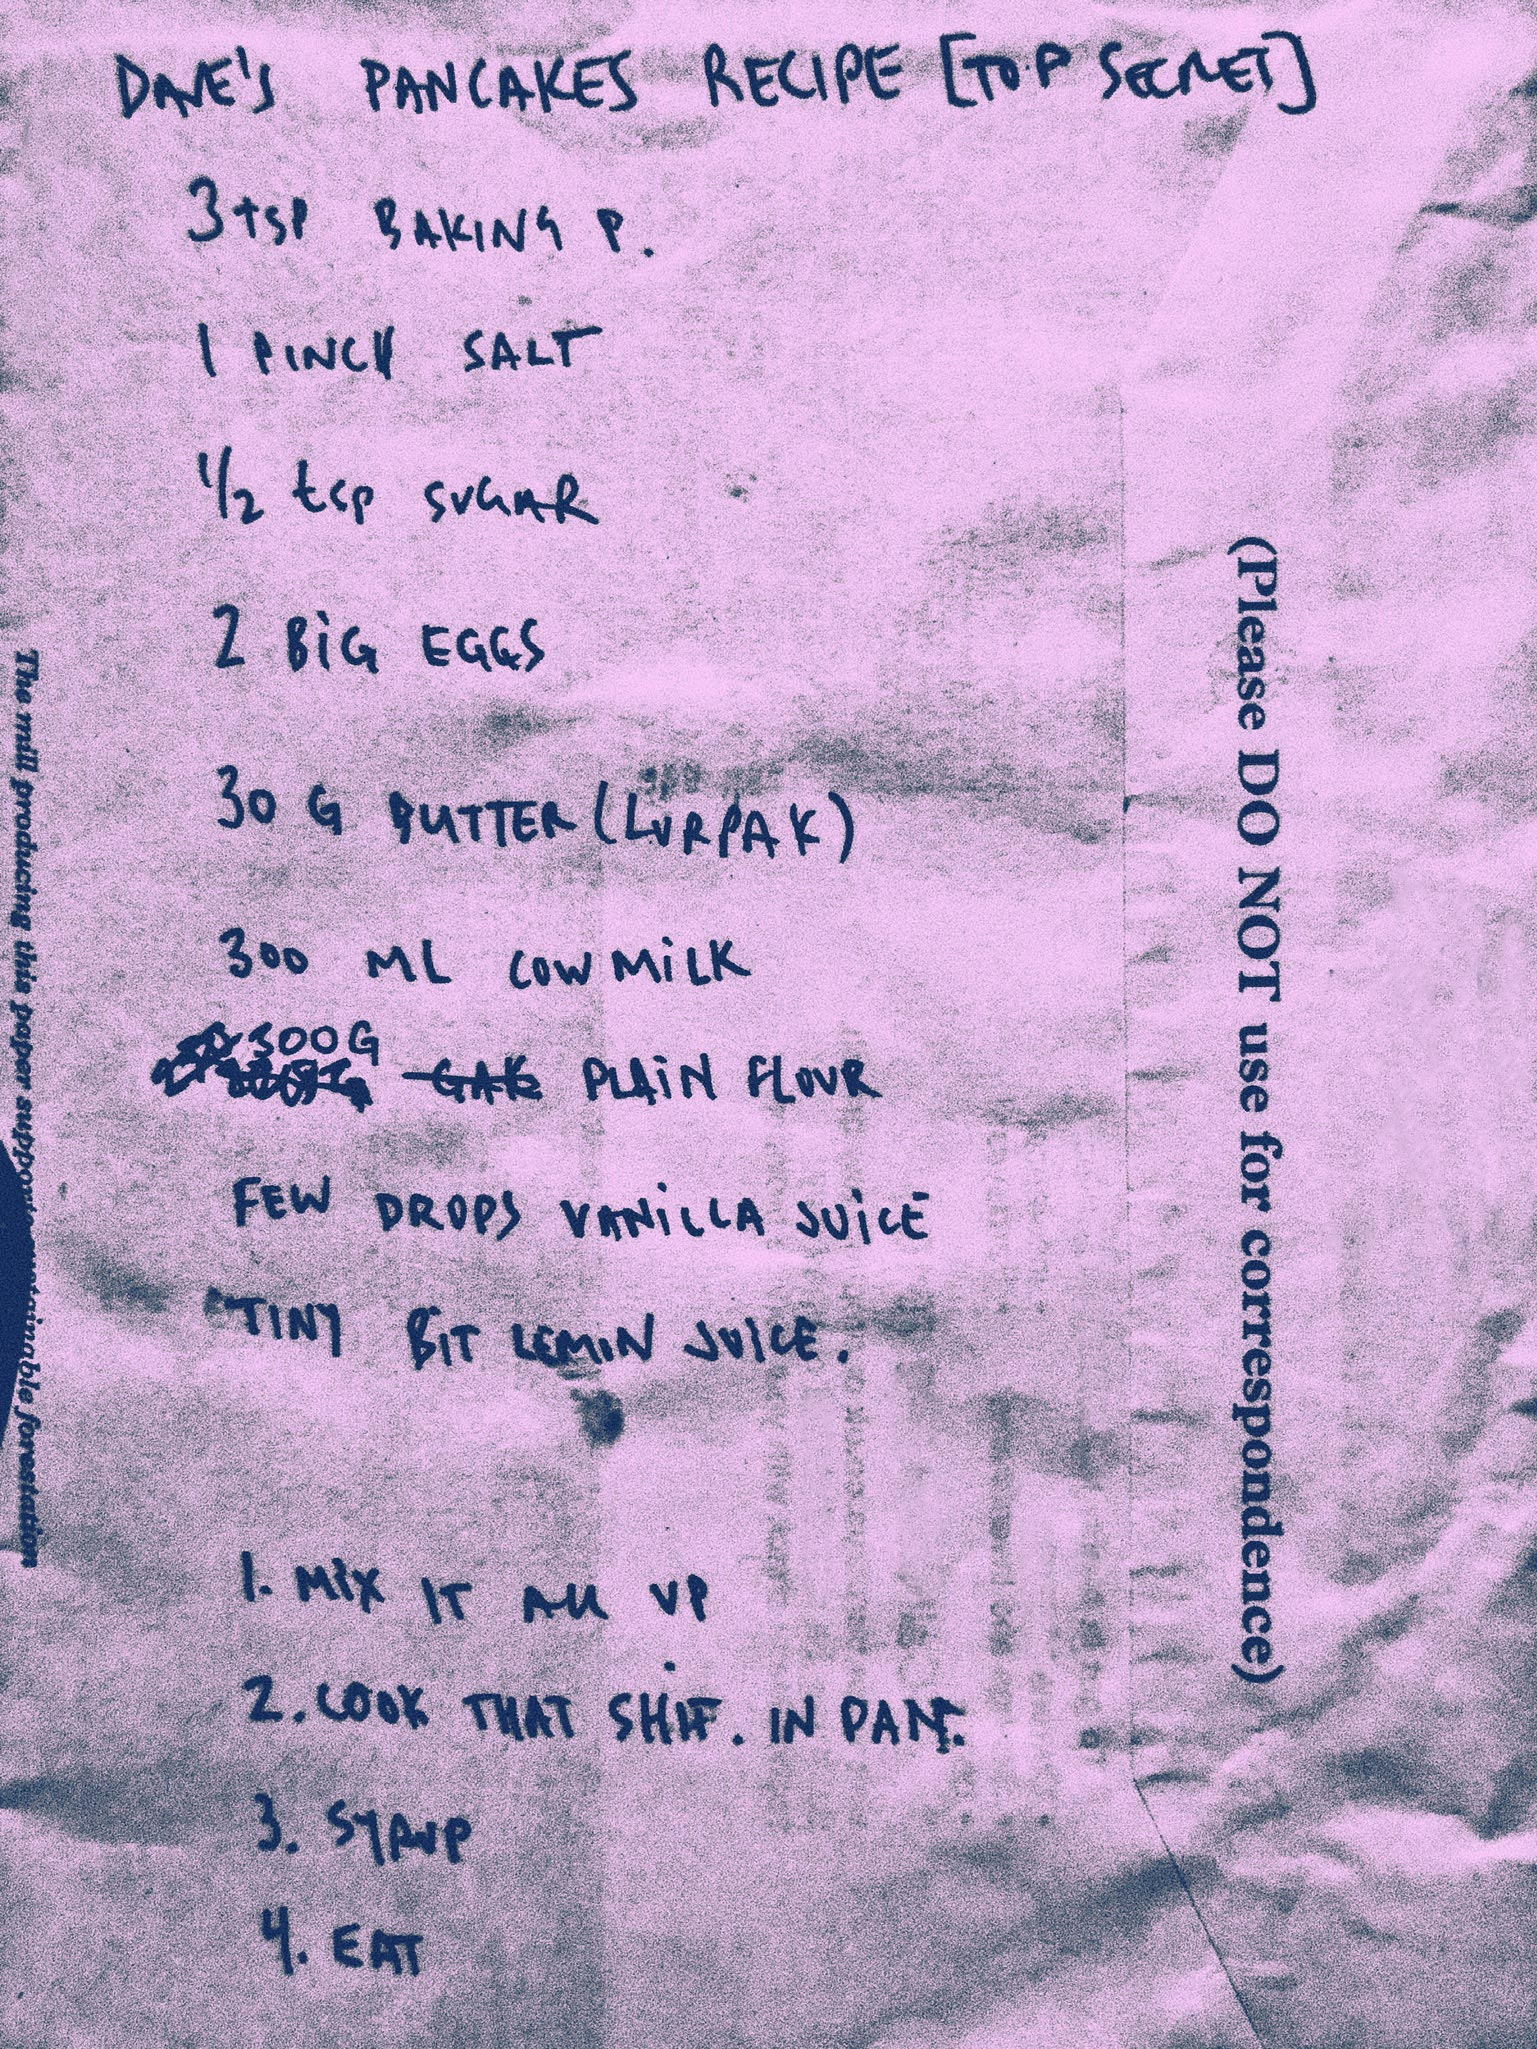
\includegraphics[width=0.5\linewidth]{graphics/DAVES_PANCAKES_RECIPE.jpg}
            \caption[cooles rezept]{Abbildung zeigt details}
    
            
            %mit label werden grafiken in texts referenziert
            \label{fig:DAVES_PANCAKES_RECIPE}
        \end{figure}
        
        \subsection {erstes Unterkapitel vom ersten Kapitel.}
        Badabing Badabum.

            \subsubsection{we need to go deeper!}

                \paragraph{insert dumb Inception joke inside the paragraph. it won't go deeper though.} 
                   
                    \subparagraph{subparagraph as smallest unit of text.}


                    
        